%%%%%%%%%%%%%%%%%%%%%%%%%%%%%%%%%%%%%%%%%%%%%%%%%%%
%
%  New template code for TAMU Theses and Dissertations starting Fall 2012.  
%  For more info about this template or the 
%  TAMU LaTeX User's Group, see http://www.howdy.me/.
%
%  Author: Wendy Lynn Turner 
%
%%%%%%%%%%%%%%%%%%%%%%%%%%%%%%%%%%%%%%%%%%%%%%%%%%%

\documentclass[12pt]{report}
\usepackage[letterpaper]{geometry}
\geometry{verbose,tmargin=1.25in,bmargin=1.25in,lmargin=1.4in,rmargin=1.15in}
 \usepackage[doublespacing]{setspace}
 \usepackage{tocloft}
 \usepackage[rm, tiny,center, compact]{titlesec}
 \usepackage{indentfirst}
 \usepackage{etoolbox}
\usepackage{tocvsec2}
 \usepackage[titletoc]{appendix}
 \usepackage{appendix}
 \usepackage{tamuconfig}
\usepackage{rotating}

% Added to fix issues with pdf searching in some versions of LaTeX
%\usepackage[T1]{fontenc}\usepackage{lmodern}
%%%%%%%%%%%%%%%%%%%%%%%%%%%%%

% Hyperref setup below.  You should be able to get away with using uncommenting just the first line.
%\usepackage[hidelinks]{hyperref}

% if \usepackage[hidelinks]{hyperref} doesn't work try this.
% \usepackage{hyperref}  % Hidelinks is an option that removes link visiability.  TAMU Thesis Offices prefers to not see the links. But often doesn't work.  
% 
% \hypersetup{
%     colorlinks=true,
%     linkcolor=black,
%     citecolor=black,
%     filecolor=black,
%     urlcolor=black,
% }
%%%%%%%  End of hyperref setup.  One of these two options should work, but my motto with hyperref is when in doubt, comment it out!
%%%%%%%%%  This hopefully fixes the problem with vertical spacing of section headings at the top of the page..  Commented out in 1.0.7
% \preto\section{%
% \ifnum\value{section}>0\addtocontents{toc}{\vskip-6pt}\fi
% }
% \preto\subsection{%
% \ifnum\value{subsection}=0\addtocontents{toc}{\vskip-6pt}\fi
% \ifnum\value{subsection}>0\addtocontents{toc}{\vskip-6pt}\fi
% } 
%%%%%%%%%%%%%%%%%%%%%%%%%%%%%%%%%%%%%%%%%%%%%%%%%%%%%%

\begin{document}

\renewcommand{\tamumanuscripttitle}{A Template-based Seismic Data Analytics Cloud Platform}
\renewcommand{\tamupapertype}{Dissertation}
\renewcommand{\tamufullname}{Yuzhong Yan}
\renewcommand{\tamudegree}{Master Degree}
\renewcommand{\tamuchairone}{Chair Name}
% Uncomment out the next line if you have co-chairs.  You will also need to edit the titlepage.tex file.
%\newcommand{\tamuchairtwo}{Additional Chair Name}
\renewcommand{\tamumemberone}{Dr. Lei Huang}
\newcommand{\tamumembertwo}{Dr. Yonggao Yang}
\newcommand{\tamumemberthree}{Dr. Kiranmai Ballem}
\renewcommand{\tamudepthead}{Dr. Yonggao Yang}
\renewcommand{\tamugradmonth}{August}
\renewcommand{\tamugradyear}{2015}
\renewcommand{\tamudepartment}{Department of Computer Science}


%%%%%%%%%%%%%%%%%%%%%%%%%%%%%%%%%%%%%%%%%%%%%%%%%%%
%
%  New template code for TAMU Theses and Dissertations starting Fall 2012.  
%  For more info about this template or the 
%  TAMU LaTeX User's Group, see http://www.howdy.me/.
%
%  Author: Wendy Lynn Turner 
%	 Version 1.0 
%  Last updated 8/5/2012
%
%%%%%%%%%%%%%%%%%%%%%%%%%%%%%%%%%%%%%%%%%%%%%%%%%%%

%%%%%%%%%%%%%%%%%%%%%%%%%%%%%% 
%% TITLE PAGE
%% The values get updated automatically.  Please do not make changes to this file other than adding/deleting committee members where necessary.
%%%%%%%%%%%%%%%%%%%%%%%%%%%%%%

\providecommand{\tabularnewline}{\\}



\begin{titlepage}
\begin{center}
\MakeUppercase{\tamumanuscripttitle}
\vspace{4em}

A \tamupapertype

by

\MakeUppercase{\tamufullname}

\vspace{4em}

\begin{singlespace}

Submitted to the Office of Graduate and Professional Studies of \\
Texas A\&M University \\

in partial fulfillment of the requirements for the degree of \\
\end{singlespace}

\MakeUppercase{\tamudegree}
\par\end{center}
\vspace{2em}
\begin{singlespace}
\begin{tabular}{ll}
 & \tabularnewline
& \cr
% If you have Co-Chairs comment out the 'Chair of Committee' line below and uncomment the 'Co-Chairs of Committee' line.
Chair of Committee, & \tamuchairone\tabularnewline
%Co-Chairs of Committee, & \tamuchairone\tabularnewline & \tamuchairtwo\tabularnewline
Committee Members, & \tamumemberone\tabularnewline
 & \tamumembertwo\tabularnewline
 & \tamumemberthree\tabularnewline
Head of Department, & \tamudepthead\tabularnewline

\end{tabular}
\end{singlespace}
\vspace{3em}

\begin{center}
\tamugradmonth \hspace{2pt} \tamugradyear

\vspace{3em}

Major Subject: \tamudepartment \par
\vspace{3em}
Copyright \tamugradyear \hspace{.5em}\tamufullname 
\par\end{center}
\end{titlepage}
\pagebreak{}




 % This is simply a file that formats and adds your titlepage, please do not edit this unless you have a specific need. .
%%%%%%%%%%%%%%%%%%%%%%%%%%%%%%%%%%%%%%%%%%%%%%%%%%%
%
%  New template code for TAMU Theses and Dissertations starting Fall 2012.  
%  For more info about this template or the 
%  TAMU LaTeX User's Group, see http://www.howdy.me/.
%
%  Author: Wendy Lynn Turner 
%	 Version 1.0 
%  Last updated 8/5/2012
%
%%%%%%%%%%%%%%%%%%%%%%%%%%%%%%%%%%%%%%%%%%%%%%%%%%%
%%%%%%%%%%%%%%%%%%%%%%%%%%%%%%%%%%%%%%%%%%%%%%%%%%%%%%%%%%%%%%%%%%%%%
%%                           ABSTRACT 
%%%%%%%%%%%%%%%%%%%%%%%%%%%%%%%%%%%%%%%%%%%%%%%%%%%%%%%%%%%%%%%%%%%%%

\chapter*{ABSTRACT}
\addcontentsline{toc}{chapter}{ABSTRACT} % Needs to be set to part, so the TOC doesnt add 'CHAPTER ' prefix in the TOC.

\pagestyle{plain} % No headers, just page numbers
\pagenumbering{roman} % Roman numerals
\setcounter{page}{2}

\indent Lorem ipsum dolor sit amet, consectetur adipiscing elit. Integer lectus quam, condimentum quis bibendum eu, sollicitudin eget lacus. Praesent non sodales odio. Class aptent taciti sociosqu ad litora torquent per conubia nostra, per inceptos himenaeos. Nulla ac luctus sapien. Morbi cursus sapien eget lorem fermentum hendrerit. Nam ac erat dui, in cursus velit. Vivamus hendrerit porttitor nisi, ut porttitor lorem volutpat eget. In ligula ligula, euismod ut condimentum sit amet, pulvinar sit amet diam. Pellentesque interdum, ipsum ullamcorper consequat dignissim, sem arcu egestas mauris, vitae interdum sem tortor ut ante. Nunc blandit laoreet nisi, non rutrum lorem hendrerit quis. Cras nunc diam, convallis et feugiat at, auctor id libero. Nunc facilisis massa eu eros imperdiet vestibulum. Vestibulum ante ipsum primis in faucibus orci luctus et ultrices posuere cubilia Curae; Donec non velit vitae tortor blandit semper.

Etiam vitae dolor nulla. Ut eros odio, rhoncus eget placerat vitae, elementum ac ante. Proin vitae odio eu nisl pharetra mattis. Pellentesque habitant morbi tristique senectus et netus et malesuada fames ac turpis egestas. Phasellus fermentum lacus consectetur neque consequat ullamcorper. Cras blandit urna non dui consequat molestie. Curabitur viverra nibh at nisi semper faucibus. Nam egestas mauris a enim dignissim nec consectetur tortor rutrum. Mauris at nisi in est luctus congue ut mattis est. Ut pretium, mi quis elementum cursus, ante eros suscipit ligula, ut porttitor elit leo sed turpis. Nam sed dui ligula.

 

\pagebreak{}

%%%%%%%%%%%%%%%%%%%%%%%%%%%%%%%%%%%%%%%%%%%%%%%%%%%
%
%  New template code for TAMU Theses and Dissertations starting Fall 2012.  
%  For more info about this template or the 
%  TAMU LaTeX User's Group, see http://www.howdy.me/.
%
%  Author: Wendy Lynn Turner 
%	 Version 1.0 
%  Last updated 8/5/2012
%
%%%%%%%%%%%%%%%%%%%%%%%%%%%%%%%%%%%%%%%%%%%%%%%%%%%

%%%%%%%%%%%%%%%%%%%%%%%%%%%%%%%%%%%%%%%%%%%%%%%%%%%%%%%%%%%%%%%%%%%%%%
%%                           DEDICATION
%%%%%%%%%%%%%%%%%%%%%%%%%%%%%%%%%%%%%%%%%%%%%%%%%%%%%%%%%%%%%%%%%%%%%
\chapter*{DEDICATION}
\addcontentsline{toc}{chapter}{DEDICATION}  % Needs to be set to part, so the TOC doesnt add 'CHAPTER ' prefix in the TOC.



\indent This is an optional page.  Lorem ipsum dolor sit amet, consectetur adipiscing elit. Integer lectus quam, condimentum quis bibendum eu, sollicitudin eget lacus. Praesent non sodales odio. Class aptent taciti sociosqu ad litora torquent per conubia nostra, per inceptos himenaeos. Nulla ac luctus sapien. Morbi cursus sapien eget lorem fermentum hendrerit. Nam ac erat dui, in cursus velit. Vivamus hendrerit porttitor nisi, ut porttitor lorem volutpat eget. In ligula ligula, euismod ut condimentum sit amet, pulvinar sit amet diam. Pellentesque interdum, ipsum ullamcorper consequat dignissim, sem arcu egestas mauris, vitae interdum sem tortor ut ante. Nunc blandit laoreet nisi, non rutrum lorem hendrerit quis. Cras nunc diam, convallis et feugiat at, auctor id libero. Nunc facilisis massa eu eros imperdiet vestibulum. Vestibulum ante ipsum primis in faucibus orci luctus et ultrices posuere cubilia Curae; Donec non velit vitae tortor blandit semper.

Etiam vitae dolor nulla. Ut eros odio, rhoncus eget placerat vitae, elementum ac ante. Proin vitae odio eu nisl pharetra mattis. Pellentesque habitant morbi tristique senectus et netus et malesuada fames ac turpis egestas. Phasellus fermentum lacus consectetur neque consequat ullamcorper. Cras blandit urna non dui consequat molestie. Curabitur viverra nibh at nisi semper faucibus. Nam egestas mauris a enim dignissim nec consectetur tortor rutrum. Mauris at nisi in est luctus congue ut mattis est. Ut pretium, mi quis elementum cursus, ante eros suscipit ligula, ut porttitor elit leo sed turpis. Nam sed dui ligula.


\pagebreak{}

%%%%%%%%%%%%%%%%%%%%%%%%%%%%%%%%%%%%%%%%%%%%%%%%%%%
%
%  New template code for TAMU Theses and Dissertations starting Fall 2012.  
%  For more info about this template or the 
%  TAMU LaTeX User's Group, see http://www.howdy.me/.
%
%  Author: Wendy Lynn Turner 
%	 Version 1.0 
%  Last updated 8/5/2012
%
%%%%%%%%%%%%%%%%%%%%%%%%%%%%%%%%%%%%%%%%%%%%%%%%%%%


%%%%%%%%%%%%%%%%%%%%%%%%%%%%%%%%%%%%%%%%%%%%%%%%%%%%%%%%%%%%%%%%%%%%%%
%%                           ACKNOWLEDGEMENTS
%%%%%%%%%%%%%%%%%%%%%%%%%%%%%%%%%%%%%%%%%%%%%%%%%%%%%%%%%%%%%%%%%%%%%
\chapter*{ACKNOWLEDGEMENTS}
\addcontentsline{toc}{chapter}{ACKNOWLEDGEMENTS}  % Needs to be set to part, so the TOC doesnt add 'CHAPTER ' prefix in the TOC.

Please find below the list of the persons you should acknowledged:

 

Supervisors (main and second)
Academic staff in your department
Technical staff
Academic staff
Colleagues
Institutions and organization
Companies
Family and friends

\pagebreak{}

%%%%%%%%%%%%%%%%%%%%%%%%%%%%%%%%%%%%%%%%%%%%%%%%%%%
%
%  New template code for TAMU Theses and Dissertations starting Fall 2012.  
%  For more info about this template or the 
%  TAMU LaTeX User's Group, see http://www.howdy.me/.
%
%  Author: Wendy Lynn Turner 
%	 Version 1.0 
%  Last updated 8/5/2012
%
%%%%%%%%%%%%%%%%%%%%%%%%%%%%%%%%%%%%%%%%%%%%%%%%%%%

%%%%%%%%%%%%%%%%%%%%%%%%%%%%%%%%%%%%%%%%%%%%%%%%%%%%%%%%%%%%%%%%%%%%%%
%%                           NOMENCLATURE
%%%%%%%%%%%%%%%%%%%%%%%%%%%%%%%%%%%%%%%%%%%%%%%%%%%%%%%%%%%%%%%%%%%%%

\chapter*{NOMENCLATURE}
\addcontentsline{toc}{chapter}{NOMENCLATURE}  % Needs to be set to part, so the TOC doesnt add 'CHAPTER ' prefix in the TOC.

\begin{tabular}{ll}
B/CS  & Bryan/College Station\tabularnewline
HSUS & Humane Society of the United States\tabularnewline
P & Pressure\tabularnewline
T  & Time\tabularnewline
TVA & Tennessee Valley Authority\tabularnewline
TxDOT \hfill{}\hfill{}\hfill{}\hfill{}\hfill{}\hfill{}\hfill{}\hfill{} & \multicolumn{1}{l}{Texas Department of Transportation}\tabularnewline
\end{tabular}

\vspace{2em}

This page is optional.

\pagebreak{}

%%%%%%%%%%%%%%%%%%%%%%%%%%%%%%%%%%%%%%%%%%%%%%%%%%%
%
%  New template code for TAMU Theses and Dissertations starting Fall 2012.  
%  For more info about this template or the 
%  TAMU LaTeX User's Group, see http://www.howdy.me/.
%
%  Author: Wendy Lynn Turner 
%	 Version 1.7
%  Last updated 3/24/2014
%
%%%%%%%%%%%%%%%%%%%%%%%%%%%%%%%%%%%%%%%%%%%%%%%%%%%
%%%%%%%%%%%%%%%%%%%%%%%%%%%%%%%%%%%%%%%%%%%%%%%%%%%%%%%%%%%%%%%%%%%%%%
%%       TABLE OF CONTENTS
%%%%%%%%%%%%%%%%%%%%%%%%%%%%%%%%%%%%%%%%%%%%%%%%%%%%%%%%%%%%%%%%%%%%%
% single-space sections in Table of Contents  - commented in version 1.7
%\renewcommand{\cftsecafterpnum}{\vskip0.5\baselineskip}
%\renewcommand{\cftsubsecafterpnum}{\vskip0.5\baselineskip}
%\renewcommand{\cftsubsubsecafterpnum}{\vskip0.5\baselineskip}
%%%%%%%%%%%%%%%%%%%%%%%%%%%%%%%%%%%%%%%%%%%%%%%%%%%

\phantomsection
\addcontentsline{toc}{chapter}{TABLE OF CONTENTS}  

\begin{singlespace}
\renewcommand\contentsname{\normalfont} {\centerline{TABLE OF CONTENTS}}

%\setcounter{tocdepth}{4} % This puts \subsubsection[]{×} in your List of Tables.  The default is 3.


%%%%%%%%%%%%%  Adds Page above the page number in TOC
\setlength{\cftaftertoctitleskip}{1em}
\renewcommand{\cftaftertoctitle}{%
\hfill{\normalfont {Page}\par}}



\tableofcontents

\end{singlespace}

\pagebreak{}

%%%%%%%%%%%%%%%%%%%%%%%%%%%%%%%%%%%%%%%%%%%%%%%%%%%%%%%%%%%%%%%%%%%%%%
%%                           LIST OF FIGURES
%%%%%%%%%%%%%%%%%%%%%%%%%%%%%%%%%%%%%%%%%%%%%%%%%%%%%%%%%%%%%%%%%%%%%

\phantomsection
\addcontentsline{toc}{chapter}{LIST OF FIGURES}  

\renewcommand{\cftloftitlefont}{\center\normalfont\MakeUppercase}

\setlength{\cftbeforeloftitleskip}{-12pt} %% Positions the LOF title vertically to match the chapter titles
\renewcommand{\cftafterloftitleskip}{12pt}


\renewcommand{\cftafterloftitle}{%
\\[4em]\mbox{}\hspace{2pt}FIGURE\hfill{\normalfont Page}\vskip\baselineskip}

\begingroup


\begin{center}
\begin{singlespace}
%% These values make the lof table entries appear double spaced between.
\setlength{\cftbeforechapskip}{0.4cm}
\setlength{\cftbeforesecskip}{0.30cm}
\setlength{\cftbeforesubsecskip}{0.30cm}
\setlength{\cftbeforefigskip}{0.4cm}
\setlength{\cftbeforetabskip}{0.4cm} 

\listoffigures

\end{singlespace}
\end{center}

\pagebreak{}


%%%%%%%%%%%%%%%%%%%%%%%%%%%%%%%%%%%%%%%%%%%%%%%%%%%%%%%%%%%%%%%%%%%%%%
%%                           lIST OF TABLES
%%%%%%%%%%%%%%%%%%%%%%%%%%%%%%%%%%%%%%%%%%%%%%%%%%%%%%%%%%%%%%%%%%%%%%
%
\phantomsection
\addcontentsline{toc}{chapter}{LIST OF TABLES}  

\renewcommand{\cftlottitlefont}{\center\normalfont\MakeUppercase}

\setlength{\cftbeforelottitleskip}{-12pt} %% Positions the LOT title vertically to match the chapter titles

\renewcommand{\cftafterlottitleskip}{12pt}


\renewcommand{\cftafterlottitle}{%
\\[4em]\mbox{}\hspace{4pt}TABLE\hfill{\normalfont Page}\vskip\baselineskip}

\begin{center}
\begin{singlespace}

%% These values make the lot table entries appear double spaced between.
\setlength{\cftbeforechapskip}{0.4cm}
\setlength{\cftbeforesecskip}{0.30cm}
\setlength{\cftbeforesubsecskip}{0.30cm}
\setlength{\cftbeforefigskip}{0.4cm}
\setlength{\cftbeforetabskip}{0.4cm}

\listoftables 

\end{singlespace}
\end{center}
\endgroup
\pagebreak{}  % Need this for the pagenumbering to be correct.   % This is simply a file that formats and adds your toc, lof, and lot, please do not edit this unless you have a specific need. .

%%%%%%%%%%%%%%%%%%%%%%%%%%%%%%%%%%%%%%%%%%%%%%%%%%%
%
%  New template code for TAMU Theses and Dissertations starting Fall 2012.  
%  For more info about this template or the 
%  TAMU LaTeX User's Group, see http://www.howdy.me/.
%
%  Author: Wendy Lynn Turner 
%	 Version 1.0 
%  Last updated 8/5/2012
%
%%%%%%%%%%%%%%%%%%%%%%%%%%%%%%%%%%%%%%%%%%%%%%%%%%%

%%%%%%%%%%%%%%%%%%%%%%%%%%%%%%%%%%%%%%%%%%%%%%%%%%%%%%%%%%%%%%%%%%%%%%
%%                           SECTION I
%%%%%%%%%%%%%%%%%%%%%%%%%%%%%%%%%%%%%%%%%%%%%%%%%%%%%%%%%%%%%%%%%%%%%


\pagestyle{plain} % No headers, just page numbers
\pagenumbering{arabic} % Arabic numerals
\setcounter{page}{1}


\chapter{\uppercase {Introduction and Background}}

Seismic reflection is the most important method used in the oil \& gas exploration industry. Huge amount of seismic data has already been generated and processed for several decades in such area, although there was no such big data concept at that time. In seismic data flow such as acquisition, migration and interpretation, it involves a lot of domain-specfic specialists and computer scientists to work together. Since the seismic data processing is both computation- and data-intensive, the High Performance Computing (HPC) technology was widely used in this area; The typical working flow should be: geophysicists use MATLAB to verify algorithms on small or synthetic sample data, then submit verified algorithms to computer scientists who will translate them into MPI codes that could run efficiently with actual data on cluster. Such procedure is both time-consuming and high-stakes that need much communication and iterations due to premature design or inconsistent results on sample and actual data. With the improvement of the data acquisition methods and requirements of high resolution for advance processing algorithms, the volume size of seismic data increases drastically, which is big challenge for the traditional way. In this paper, we will try to setup a seismic data processing platform on which all stakeholders could work with same data sets and algorithms or models without much performance expense.

\section{Seismic Data Processing Flow}
As a dominant method of exploration geophysics in oil \& gas area, reflection seismology (or seismic reflection) uses the principles of seismology to estimate the properties of the Earth's subsurface from reflected seismic waves \cite{seisreflection}. Although the theory of reflection is simple, but the processing flow is more sophisticated in pratical scenario. The main steps in such work flow include: data acquistion, data processing, data interpretation and attribute analysis.

In the data acquistion stage, seismic sources such as dynamite or air gun are used to generate seismic waves, and the waves are reflected or refracted while encountering different type of materials underground and are recoreded by the receivers. It becames more complicated in non-normal incidence, such as refraction, multiple reflection and cultural noise, and all these factors need to be considered in processing stage. The first stage is pre-processing after acquiring the survey data, in which main steps are removing noise and boosting signal level. Velocity analysis, stacking and migration are main tasks in seismic data processing, and after migration the seismic events are geometrically re-located in either space or time to the location the event occurred in subsurface and create a complete image of subsurface\cite{seisreflection}. The main goal of seismic interpretation is trying to find petroleum reservoir. But such task requires deep analysis of seismic attributes and geophysics related knowledge, and involves huge amount human resource such as computer scientists, geologists and geophysicists etc. In this paper, we focus on latter stage and built a platform that facilitates seismic attributes extraction and analytics.   

\begin{figure}[h]
\centering
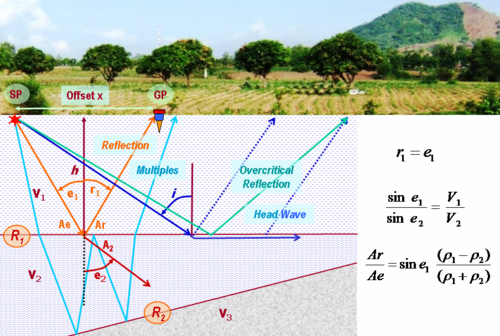
\includegraphics[scale=1]{figures/seismic_reflection_principal.png}
\caption{Seismic Reflection Outlines\cite{seisreflection}}
\label{seismic_reflection}
\end{figure}

%A landscape figure should be shown below. 
%%%%%%%%%%%%%%%%%%%%%%%%%%%%%%%%%%%%%%%%%%%%%%%%%%%%%%
%\begin{sidewaysfigure}[H]
%\centering
%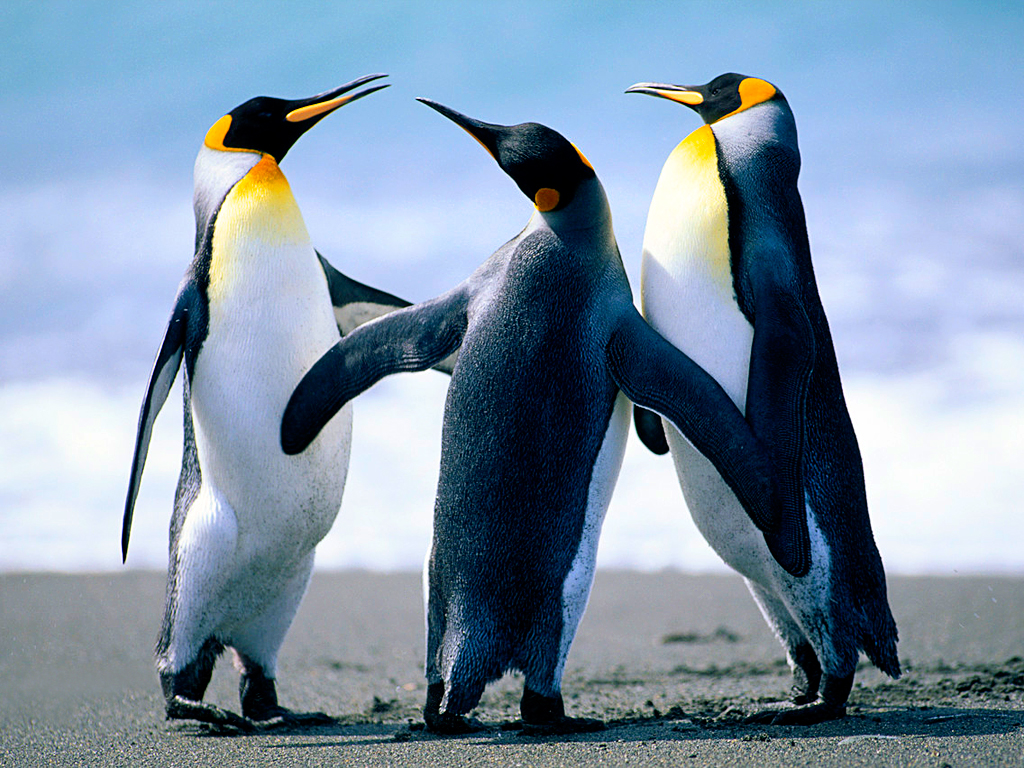
\includegraphics[scale=.50]{figures/Penguins.jpg}
%\caption{TAMU figure - This is an example of a long figure title with a landscape figure.  Figure titles need to be single-spaced within and double spaced between in the list of figures.}
%\label{fig:tamu-fig1-1}
%\end{sidewaysfigure}
%%%%%%%%%%%%%%%%%%%%%%%%%%%%%%%%%%%%%%%%%%%%%%%%%%%%%%


\section{Current Processing Methodlogy}
HPC technology has been used to process seismic data for several decades. In most current big oil \& gas companies or related service companies, there must have an IT department and a huge group of geophysicists or data scientists forming the research teams. In normal case, each small team set up a research project, and then develop new models or algorithms to verify their idea. In this stage, they only use synthetic or historical small data to do experiments, and their programming environment is MATLAB in general. But why did not they experimentalize on big cluster with actual seismic data? The main reason is that geophysicists are not familiar with HPC environment, and their main target is to verify the validity of algorithms or models, but not the performance. The volume size of actual data is usually very large and will take much more time to run with MATLAB codes. After research work was finished and got approval, geophysicists will submit their MATLAB codes to IT department, and then experts in HPC domain will translate such codes into MPI codes or hybrid OpenMP/MPI codes and verify them on high performance cluster with actual seismic data. If there are any problems in such stage, the original authors need to be involved to find the root cause together, and the results were either changing algorithms\/models by geophysicists or modification of programming implementation. To make such a research project become a mature product, it will often take one more year with several iterations.

%\subsection{This is a Very Long Subsection Title This is a Very Long Subsection Title}


\section{The Big Challeges}
In fact, there are problems in current seismic data analytics flow. As shown in previous section, the MATLAB codes work well on sample data do not mean they could run successfully in parallel after translating into MPI codes. The test cases on MATLAB codes are usually not enough, and the parallization itself may also produce new problems. The biggest challege from now on is burst increase of data volume size, which also need more advance algorithms and models to process. For instance, the volume size of high dimension such as 3D even 4D seismic data and high density seismic data are growing exponentially, so seismic data processing becomes both computation- and data- intensive problems. The traditional HPC programming model is good at handle computation intense case, but for huge increase of volume size, data movement between nodes is the greatest bottleneck even with infiniband connections. Another problem is the maintainence and reuse of legacy codes; Most of HPC codes in such area were written in Fortran to achieve high performance, the readability and maintenance of such programs are also challeges for beginners or successors. With the improvement of CPU computation power and programming architecture, we should not only focus on executation time, but also the overall performance of whole company and entire industry. 


%%%%%%%%%%%%%%%%%%%%%%%%%%%%%%%%%%%%%%%%%%%%%%%%%%%
%
%  New template code for TAMU Theses and Dissertations starting Fall 2012.  
%  For more info about this template or the 
%  TAMU LaTeX User's Group, see http://www.howdy.me/.
%
%  Author: Wendy Lynn Turner 
%	 Version 1.0 
%  Last updated 8/5/2012
%
%%%%%%%%%%%%%%%%%%%%%%%%%%%%%%%%%%%%%%%%%%%%%%%%%%%

%%%%%%%%%%%%%%%%%%%%%%%%%%%%%%%%%%%%%%%%%%%%%%%%%%%%%%%%%%%%%%%%%%%%%%%
%%%                           SECTION II
%%%%%%%%%%%%%%%%%%%%%%%%%%%%%%%%%%%%%%%%%%%%%%%%%%%%%%%%%%%%%%%%%%%%%%

\chapter{\uppercase {Literature Review: The Importance of Research Part Two- This is designed to test long titles in the TOC}}

Text goes here.

\section{New Section}
%%%%%%%%%%%%%%%%%%%%%%%%%%%%%%%%%%%%%%%%%%%%%%%%%%%%%%
\begin{figure}[H]
\centering
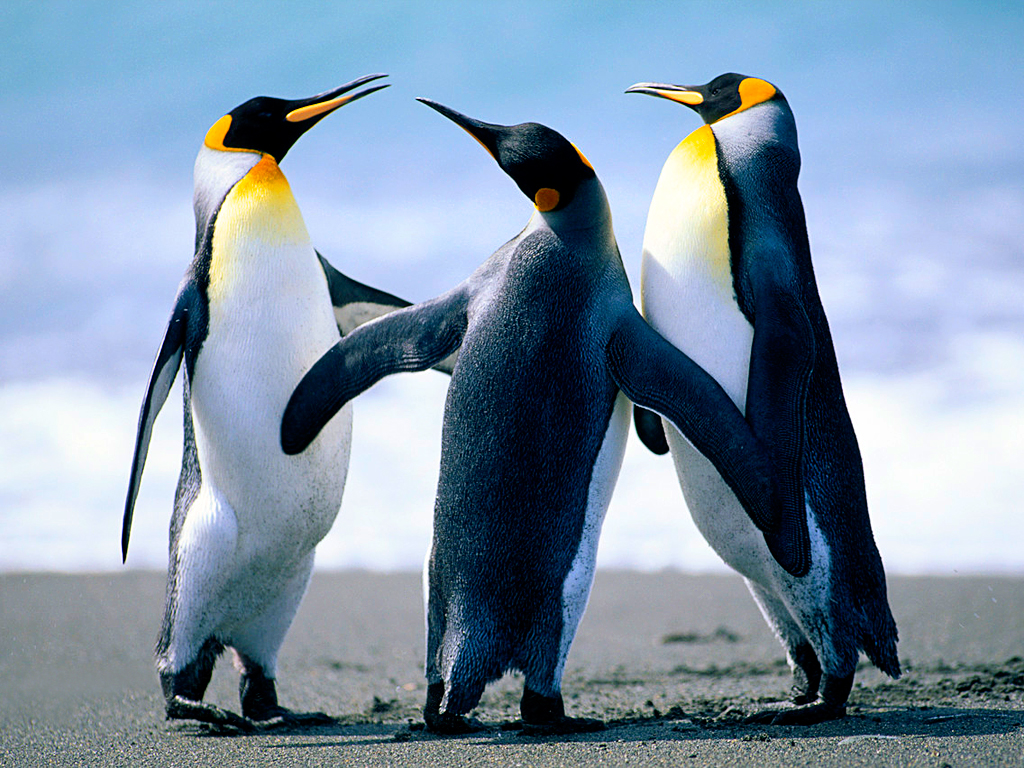
\includegraphics[scale=.50]{figures/Penguins.jpg}
\caption{TAMU figure - This is an example of a long figure title.  Figure titles need to be single-spaced within and double spaced between in the list of figures.}
\label{fig:landscapepenguins}
\end{figure}
%%%%%%%%%%%%%%%%%%%%%%%%%%%%%%%%%%%%%%%%%%%%%%%%%%%%%%
\subsection{Subsection}
\begin{table}[H]
\centering
\caption{This is a table template - This is an example of a long table title.  Table titles need to be single-spaced within and double spaced between in the list of tables.}
\begin{tabular}{|l|c|c|c|c|c|}
\hline
Product & 1 & 2 & 3 & 4 & 5\\
\hline
Price & 124.- & 136.- & 85.- & 156.- & 23.-\\
Guarantee [years] & 1 & 2 & - & 3 & 1\\
Rating & 89\% & 84\% & 51\% & & 45\%\\
\hline
\hline
Recommended & yes & yes & no & no & no\\
\hline
\end{tabular}
\label{tab:template1}
\end{table}


\subsection{Subsection}
%%%%%%%%%%%%%%%%%%%%%%%%%%%%%%%%%%%%%%%%%%%%%%%%%%%%%%
\begin{figure}[H]
\centering
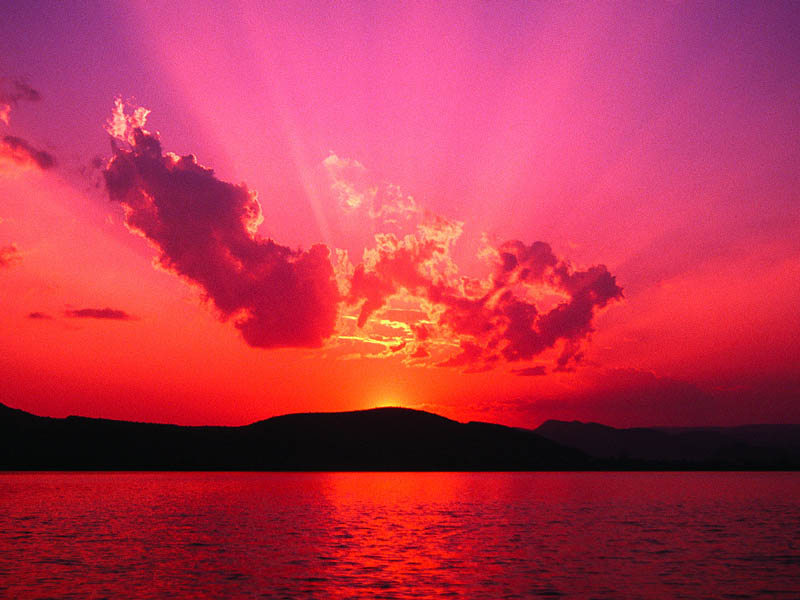
\includegraphics[scale=.50]{figures/Sunset.jpg}
\caption{Sunset figure}
\label{fig:sunset-fig2}
\end{figure}
%%%%%%%%%%%%%%%%%%%%%%%%%%%%%%%%%%%%%%%%%%%%%%%%%%%%%%
\subsubsection{This is a subsubsection}
\begin{table}[H]
\centering
\caption{This is a table template - This is an example of a long table title.  Table titles need to be single-spaced within and double spaced between in the list of tables.}
\begin{tabular}{|l|c|c|c|c|c|}
\hline
Product & 1 & 2 & 3 & 4 & 5\\
\hline
Price & 124.- & 136.- & 85.- & 156.- & 23.-\\
Guarantee [years] & 1 & 2 & - & 3 & 1\\
Rating & 89\% & 84\% & 51\% & & 45\%\\
\hline
\hline
Recommended & yes & yes & no & no & no\\
\hline
\end{tabular}
\label{tab:template1-2}
\end{table}
\section{Another Section}

%%%%%%%%%%%%%%%%%%%%%%%%%%%%%%%%%%%%%%%%%%%%%%%%%%%
%
%  New template code for TAMU Theses and Dissertations starting Fall 2012.  
%  For more info about this template or the 
%  TAMU LaTeX User's Group, see http://www.howdy.me/.
%
%  Author: Wendy Lynn Turner 
%	 Version 1.0 
%  Last updated 8/5/2012
%
%%%%%%%%%%%%%%%%%%%%%%%%%%%%%%%%%%%%%%%%%%%%%%%%%%%
%%%%%%%%%%%%%%%%%%%%%%%%%%%%%%%%%%%%%%%%%%%%%%%%%%%%%%%%%%%%%%%%%%%%%%
%%                           SECTION III
%%%%%%%%%%%%%%%%%%%%%%%%%%%%%%%%%%%%%%%%%%%%%%%%%%%%%%%%%%%%%%%%%%%%%



\chapter{\uppercase{Related work}}

Text goes here \cite{ApacheHadoop}.

\section{Apache Hadoop}

%%%%%%%%%%%%%%%%%%%%%%%%%%%%%%%%%%%%%%%%%%%%%%%%%%%%%%
\begin{figure}[H]
\centering
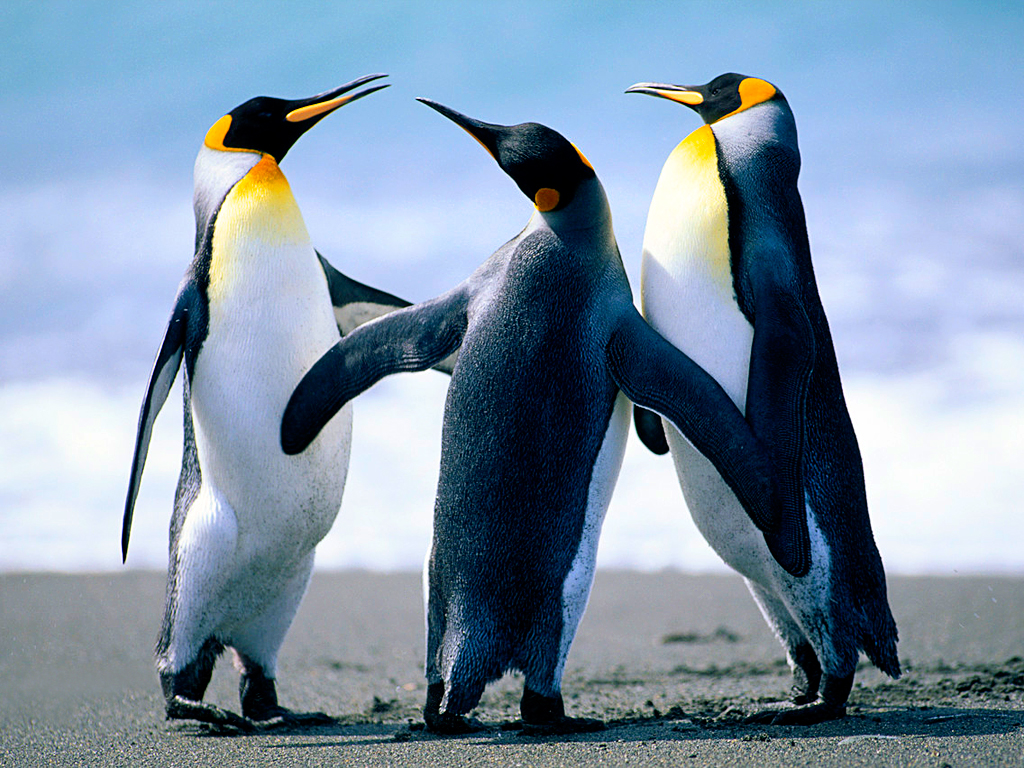
\includegraphics[scale=.50]{figures/Penguins.jpg}
\caption{TAMU figure}
\label{fig:tamu-fig3}
\end{figure}
%%%%%%%%%%%%%%%%%%%%%%%%%%%%%%%%%%%%%%%%%%%%%%%%%%%%%%
\section{Apache Spark}

Text between the figures.  Text between the figures. Text between the figures. Text between the figures.  Text between the figures. Text between the figures. Text between the figures.  Text between the figures. Text between the figures. Text between the figures.  Text between the figures. Text between the figures.
%%%%%%%%%%%%%%%%%%%%%%%%%%%%%%%%%%%%%%%%%%%%%%%%%%%%%%%
%\begin{figure}[H]
%\centering
%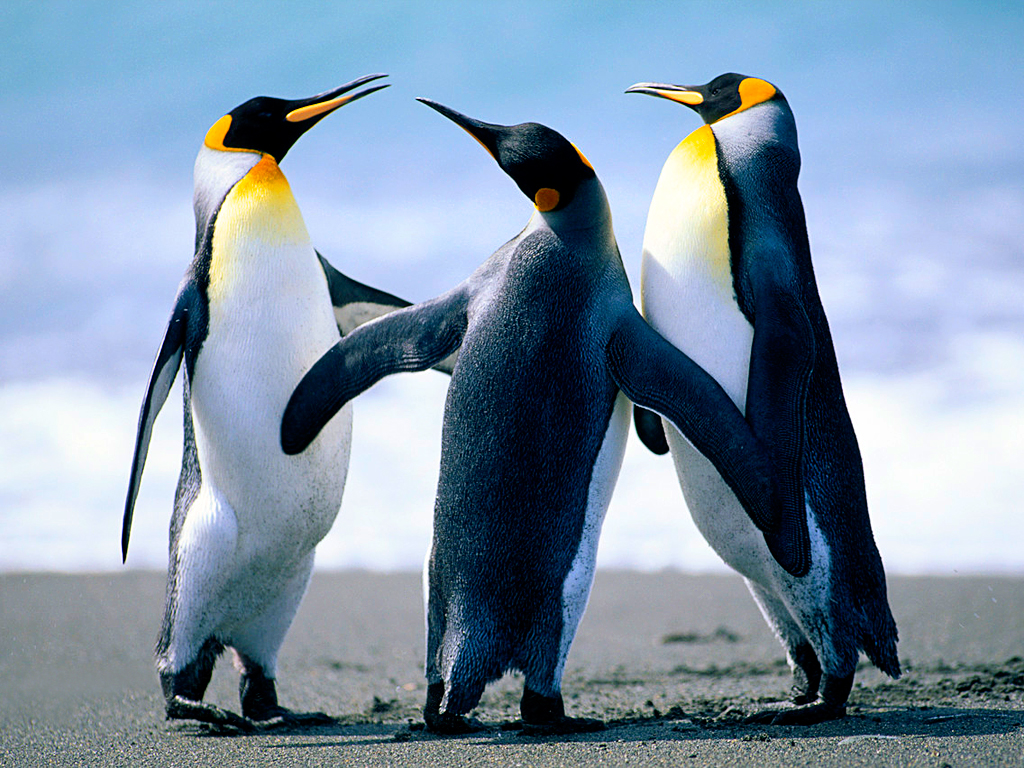
\includegraphics[scale=.50]{figures/Penguins.jpg}
%\caption{Another TAMU figure}
%\label{fig:tamu-fig4}
%\end{figure}
%%%%%%%%%%%%%%%%%%%%%%%%%%%%%%%%%%%%%%%%%%%%%%%%%%%%%%%

\subsection{Subsection}

%%%%%%%%%%%%%%%%%%%%%%%%%%%%%%%%%%%%%%%%%%%%%%%%%%%%%%%
%\begin{figure}[H]
%\centering
%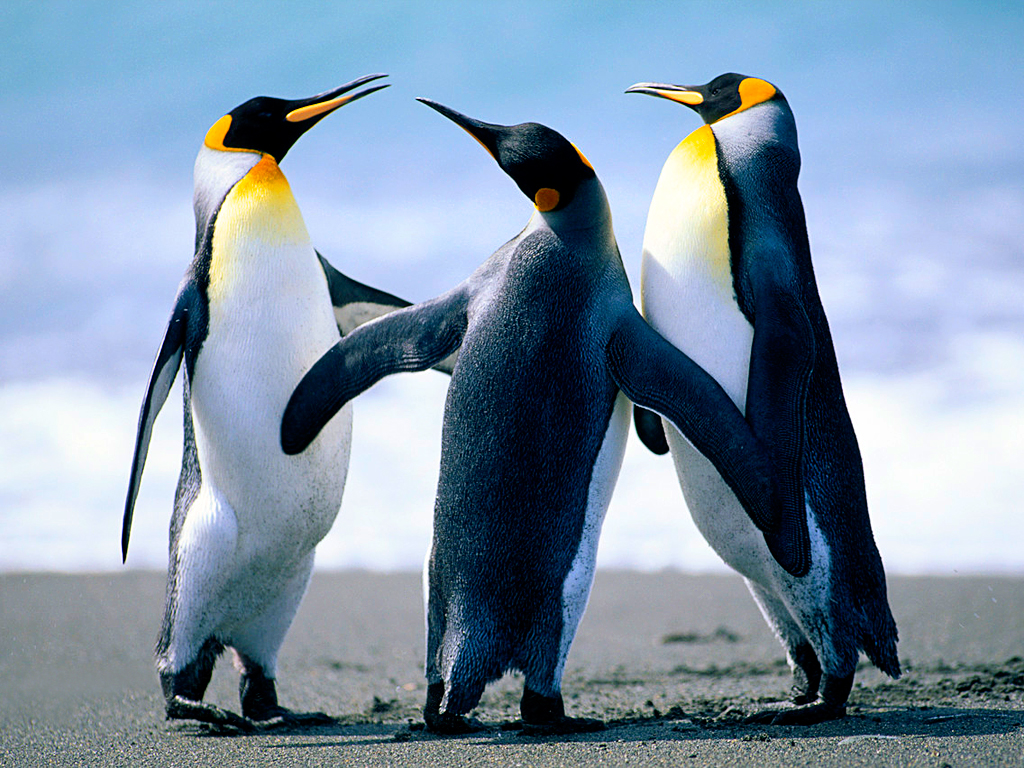
\includegraphics[scale=.50]{figures/Penguins.jpg}
%\caption{Another TAMU figure}
%\label{fig:tamu-fig4-2}
%\end{figure}
%%%%%%%%%%%%%%%%%%%%%%%%%%%%%%%%%%%%%%%%%%%%%%%%%%%%%%%
\subsection{Subsection}

A table example is going to follow.

\begin{table}[H]
\centering
\caption{This is a table template}
\begin{tabular}{|l|c|c|c|c|c|}
\hline
Product & 1 & 2 & 3 & 4 & 5\\
\hline
Price & 124.- & 136.- & 85.- & 156.- & 23.-\\
Guarantee [years] & 1 & 2 & - & 3 & 1\\
Rating & 89\% & 84\% & 51\% & & 45\%\\
\hline
\hline
Recommended & yes & yes & no & no & no\\
\hline
\end{tabular}
\label{tab:template2}
\end{table}
\subsubsection{This is a subsubsection}

\section{Python}





fix spacing in bibliography, if any...
%%%%%%%%%%%%%%%%%%%%%%%%%%%%%%%%%%%%%%%%%%%%%%%%%%%%%%%%%%%%%
\let\oldbibitem\bibitem
\renewcommand{\bibitem}{\setlength{\itemsep}{0pt}\oldbibitem}
%%%%%%%%%%%%%%%%%%%%%%%%%%%%%%%%%%%%%%%%%%%%%%%%%%%%%%%%%%%%%%%
%%%%%%%%%%%%%%%%%%%%%%%%%%%%%%%%%%%%%%%%%%%%%%%%%%%
%
%  New template code for TAMU Theses and Dissertations starting Fall 2012.  
%  For more info about this template or the 
%  TAMU LaTeX User's Group, see http://www.howdy.me/.
%
%  Author: Wendy Lynn Turner 
%	 Version 1.0 
%  Last updated 8/5/2012
%
%%%%%%%%%%%%%%%%%%%%%%%%%%%%%%%%%%%%%%%%%%%%%%%%%%%


%%%%%%%%%%%%%%%%%%%%%%%%%%%%%%%%%%%%%%%%%%%%%%%%%%%%%%%%%%%%%%%%%%%%%%
%%                           REFERENCES 
%%%%%%%%%%%%%%%%%%%%%%%%%%%%%%%%%%%%%%%%%%%%%%%%%%%%%%%%%%%%%%%%%%%%%

\phantomsection
\addcontentsline{toc}{chapter}{REFERENCES}

\renewcommand{\bibname}{{\large\textbf\center REFERENCES}}

\bibliographystyle{plain}
\bibliography{references}

% %%%%%%%%%%%%%%%%%%%%%%%%%%%%%%%%%%%%%%%%%%%%%%%%%%%
%
%  New template code for TAMU Theses and Dissertations starting Fall 2012.  
%  For more info about this template or the 
%  TAMU LaTeX User's Group, see http://www.howdy.me/.
%
%  Author: Wendy Lynn Turner 
%	 Version 1.0 
%  Last updated 8/5/2012
%
%%%%%%%%%%%%%%%%%%%%%%%%%%%%%%%%%%%%%%%%%%%%%%%%%%%

\begin{appendices}
\titleformat{\chapter}{\centering\normalsize}{APPENDIX \thechapter}{0em}{\vskip .5\baselineskip\centering}
\renewcommand{\appendixname}{APPENDIX}

%%%%%%%%%%%%%%%%%%%%%%%%%%%%%%%%%%%%%%%%%%%%%%%%%%%
%
%  New template code for TAMU Theses and Dissertations starting Fall 2012.  
%  For more info about this template or the 
%  TAMU LaTeX User's Group, see http://www.howdy.me/.
%
%  Author: Wendy Lynn Turner 
%	 Version 1.0 
%  Last updated 8/5/2012
%
%%%%%%%%%%%%%%%%%%%%%%%%%%%%%%%%%%%%%%%%%%%%%%%%%%%

%%%%%%%%%%%%%%%%%%%%%%%%%%%%%%%%%%%%%%%%%%%%%%%%%%%%%%%%%%%%%%%%%%%%%%
%%                           APPENDIX A 
%%%%%%%%%%%%%%%%%%%%%%%%%%%%%%%%%%%%%%%%%%%%%%%%%%%%%%%%%%%%%%%%%%%%%

\phantomsection

\chapter{\uppercase{First Appendix}}

Text for the Appendix follows.

\begin{figure}[H]
\centering
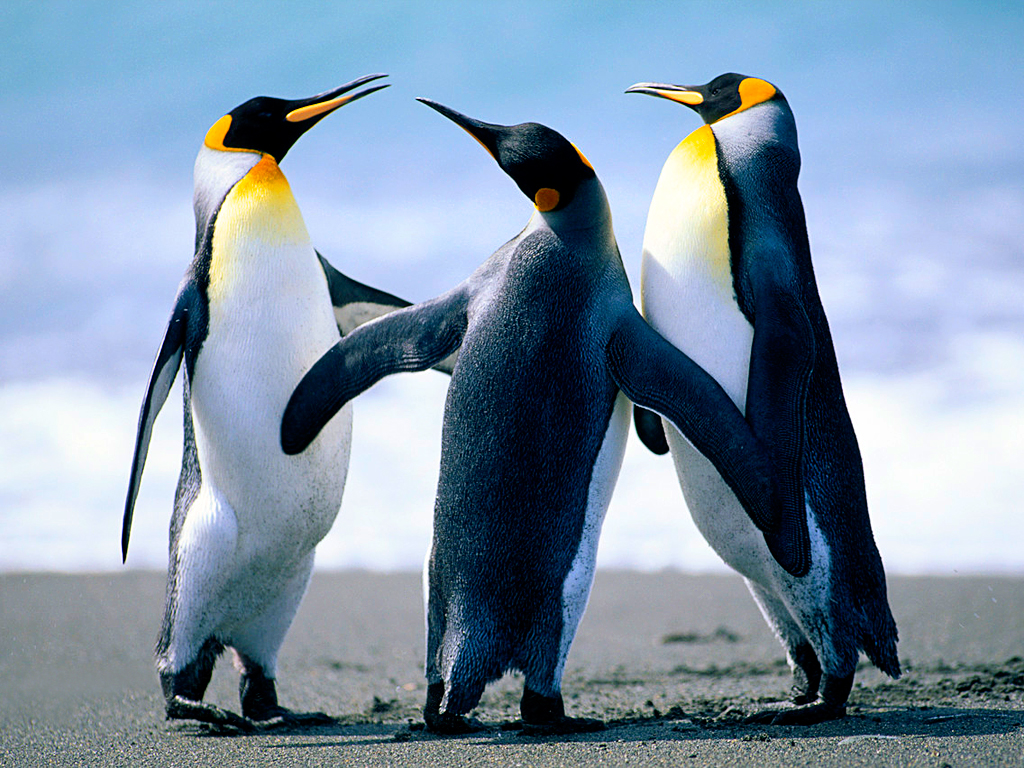
\includegraphics[scale=.50]{figures/Penguins.jpg}
\caption{TAMU figure}
\label{fig:tamu-fig5}
\end{figure}

%%%%%%%%%%%%%%%%%%%%%%%%%%%%%%%%%%%%%%%%%%%%%%%%%%%
%
%  New template code for TAMU Theses and Dissertations starting Fall 2012.  
%  For more info about this template or the 
%  TAMU LaTeX User's Group, see http://www.howdy.me/.
%
%  Author: Wendy Lynn Turner 
%	 Version 1.0 
%  Last updated 8/5/2012
%
%%%%%%%%%%%%%%%%%%%%%%%%%%%%%%%%%%%%%%%%%%%%%%%%%%%

%%%%%%%%%%%%%%%%%%%%%%%%%%%%%%%%%%%%%%%%%%%%%%%%%%%%%%%%%%%%%%%%%%%%%%
%%                           APPENDIX B
%%%%%%%%%%%%%%%%%%%%%%%%%%%%%%%%%%%%%%%%%%%%%%%%%%%%%%%%%%%%%%%%%%%%%

\chapter{\uppercase {Second Appendix with a longer title - much longer in fact}}

Text for the Appendix follows.

\begin{figure}[H]
\centering
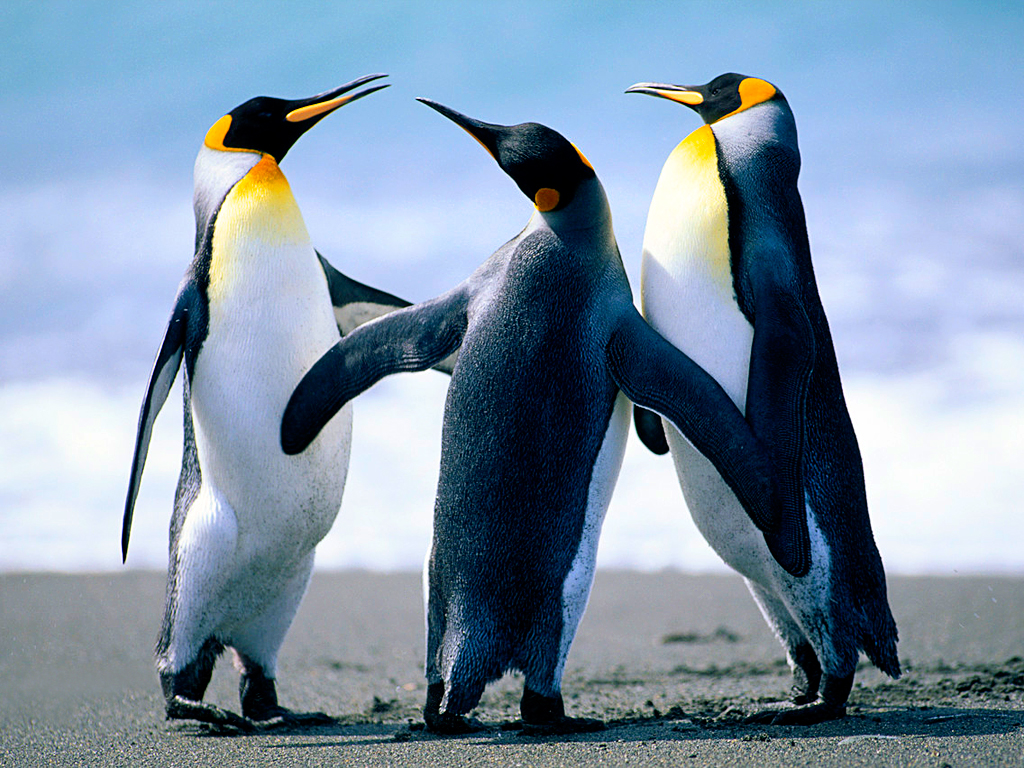
\includegraphics[scale=.50]{figures/Penguins.jpg}
\caption{TAMU figure}
\label{fig:tamu-fig6}
\end{figure}

\section{Appendix Section}


\pagebreak{}

\end{appendices}



\end{document}
